\section[The Cosmic Microwave Background]{\hyperlink{toc}{The Cosmic Microwave Background}}

\subsection{Baryon-to-Photon Ratio and Recombination Temperature}
We recall the fractional ionization as solved for using the Saha equation:
\begin{equation}
    X = \frac{-1 + \sqrt{1 + 4S}}{2S}
\end{equation}
where $S$ is given by:
\begin{equation}
    S(T, \eta) = 3.84\eta\left(\frac{kT}{m_e c^2}\right)^{3/2}\exp(\frac{Q}{kT})
\end{equation}
where $T$ is the temperature, $\eta$ is the baryon-to-photon ratio, and $Q$ is the ionization energy. We take $k = 8.62 \times 10^{-5}\si{eV.K^{-1}}$, $Q = 13.6\si{eV}$, $m_e c^2 = 511000\si{eV}$. For $\eta = 4 \times 10^{-10}$ and for $\eta = 8 \times 10^{-10}$, we get:
\begin{figure}[htbp]
    \centering
    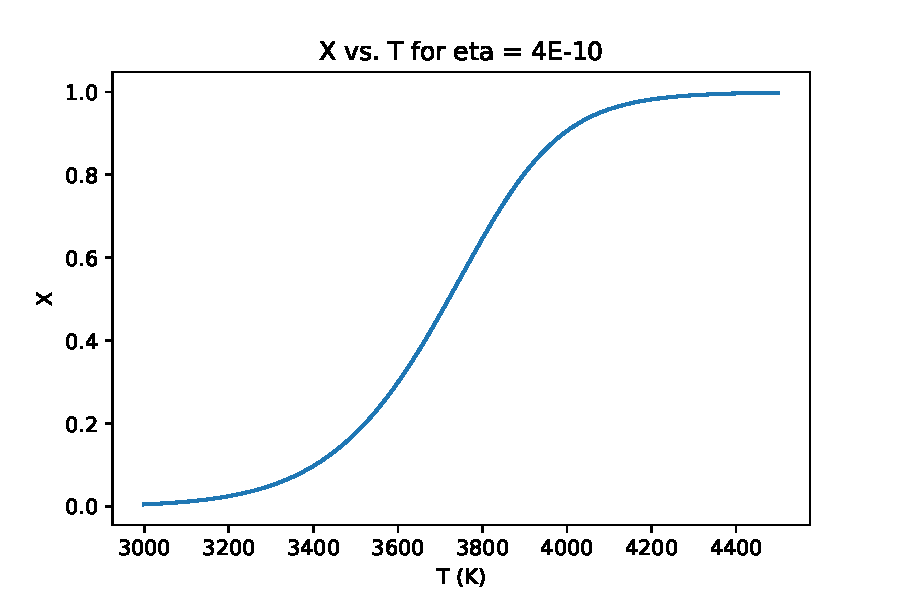
\includegraphics[scale=0.52]{Images/Q8-1eta4.pdf}
    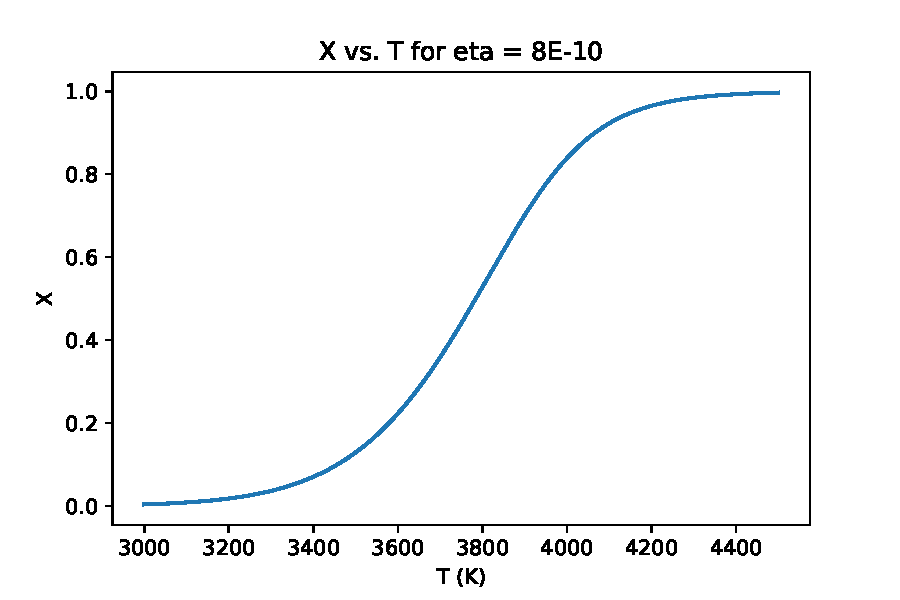
\includegraphics[scale=0.52]{Images/Q8-1eta8.pdf}
    
    \caption{Plots of fractional ionization $X$ as a function of temperature $T$ (in Kelvin) for baryon-to-photon ratios $\eta = 4 \times 10^{-10}$ and $\eta = 8 \times 10^{-10}$.}
    \label{fig-Q81}
\end{figure}

Taking $T_{\text{rec}}$ to be when $X = 1/2$, for $\eta = 4 \times 10^{-10}$, we have $\boxed{T_{\text{rec}} = 3720\si{K}}$, and for $\eta = 8 \times 10^{-10}$, we have $\boxed{T_{\text{rec}} = 3784\si{K}}$. Doubling the photon-to-baryon ratio has a small effect (only a relative change of about $1.7\%$).

\subsection{}
\subsection{}
\subsection{}